\documentclass[12pt,a4paper]{article}

% --- Packages de base ---
\usepackage[utf8]{inputenc}
\usepackage[french]{babel}
\usepackage[T1]{fontenc}
\usepackage{geometry}
\geometry{hmargin=2.5cm,vmargin=2.5cm}

% --- Graphiques et Tableaux ---
\usepackage{graphicx}
\usepackage{booktabs}
\usepackage{array}

% --- Liens et Code ---
\usepackage{hyperref}
\hypersetup{
    colorlinks=true,
    linkcolor=blue,
    urlcolor=blue,
    pdftitle={Compte Rendu - Test d'Injection SQL}
}
\usepackage{listings}
\usepackage{xcolor}

% --- Configuration de Listings pour le Code Python/SQL ---
\definecolor{codegreen}{rgb}{0,0.6,0}
\definecolor{codegray}{rgb}{0.5,0.5,0.5}
\definecolor{codepurple}{rgb}{0.58,0,0.82}
\definecolor{backcolour}{rgb}{0.95,0.95,0.92}

\lstdefinestyle{mystyle}{
    backgroundcolor=\color{backcolour},   
    commentstyle=\color{codegreen},
    keywordstyle=\color{magenta},
    numberstyle=\tiny\color{codegray},
    stringstyle=\color{codepurple},
    basicstyle=\ttfamily\footnotesize,
    breakatwhitespace=false,         
    breaklines=true,                 
    captionpos=b,                    
    keepspaces=true,                 
    numbers=left,                    
    numbersep=5pt,                  
    showspaces=false,                
    showstringspaces=false,
    showtabs=false,                  
    tabsize=2
}
\lstset{style=mystyle}

\begin{document}

% --- Page de Garde ---
\begin{titlepage}
    \centering
    \vspace*{1cm}
    
    {\Large \textbf{UNIVERSITÉ DE HAUTE-ALSACE}}\\[0.3cm]
    {\large Master IM (Informatique et Mobilité)}\\[0.2cm]
    {\large Année Universitaire 2026 -- 2027}\\[2.5cm]
    
    \rule{\linewidth}{0.5mm}\\[0.5cm]
    {\huge \bfseries COMPTE RENDU DE TP}\\[0.3cm]
    {\Large \textbf{Sécurisation des Applications : Injections SQL}}\\[0.5cm]
    \rule{\linewidth}{0.5mm}\\[3cm]
    
    \begin{minipage}{0.45\textwidth}
        \begin{flushleft} \large
            \textbf{Réalisé par :}\\
            Nourine Abdelmalek\\
            \textit{Étudiant M2 IM}
        \end{flushleft}
    \end{minipage}
    ~
    \begin{minipage}{0.45\textwidth}
        \begin{flushright} \large
            \textbf{Encadré par :}\\
            Prof. Hammoudi Karim\\
            \textit{Enseignant-chercheur}
        \end{flushright}
    \end{minipage}
    
    \vfill
    
    {\large \today}
\end{titlepage}

\newpage
\tableofcontents
\newpage

% --------------------------------------------------
\section{Introduction}
% --------------------------------------------------
L'objectif de ce compte rendu est de tester la présence éventuelle de failles d'injection SQL dans une application web développée en \textbf{Python (Flask)} pour la gestion des projets d'une entreprise.

L'application est exécutée localement sur l'environnement de développement. Elle utilise Python pour la partie serveur Web et une base de données relationnelle (\textbf{SQLite / PostgreSQL}) pour stocker les informations relatives aux projets, employés, managers, budgets et affectations.

Les tests sont réalisés uniquement sur l'environnement local du projet à l'adresse \texttt{http://127.0.0.1:5000}.

% --------------------------------------------------
\section{Présentation de l'application}
% --------------------------------------------------
L'application étudiée permet de gérer :
\begin{itemize}
    \item Les projets (nom du projet, manager du projet, budget, date de début) ;
    \item Les employés (identifiant, nom, salaire annuel) ;
    \item Les départements et managers hiérarchiques ;
    \item Les affectations d'employés aux projets (nombre d'heures par semaine, évaluation).
\end{itemize}

L'application est accessible localement à l'adresse :
\begin{center}
    \url{http://127.0.0.1:5000/}
\end{center}

La table principale au cœur de l'application est la relation \texttt{Projet} qui contient le schéma suivant :
\begin{center}
\small
\texttt{Projet(nomProj, mgrProj, idEmp, heures, nomEmp, budget, dateDebut, salEmp, mgrEmp, deptEmp, evalEmp)}
\end{center}

La recherche d'affectations s'effectue via le champ de recherche de la page d'accueil avec le paramètre GET \texttt{q}.

% --------------------------------------------------
\section{Objectif du test d'injection SQL}
% --------------------------------------------------
Une injection SQL (\textit{SQL Injection - SQLi}) est une vulnérabilité critique qui survient lorsqu'une application web construit une requête SQL dynamique en concaténant directement des données saisies par l'utilisateur sans neutralisation préalable.

L'objectif du test est de vérifier si les paramètres transmis à l'application (notamment le champ de recherche \texttt{q}) permettent de modifier le comportement de la requête exécutée par le SGBD, soit pour accéder à des données non autorisées, soit pour provoquer des erreurs de syntaxe SQL.

% --------------------------------------------------
\section{Test avec une valeur normale}
% --------------------------------------------------
Dans un premier temps, nous effectuons un test fonctionnel avec une valeur normale correspondant à un projet existant dans la base de données.

L'URL utilisée est :
\begin{center}
    \url{http://127.0.0.1:5000/?q=ILO}
\end{center}

Le paramètre \texttt{q} contient ici la valeur \texttt{ILO}.

\subsection{Résultat}
Le projet \texttt{ILO} existe dans la base de données (associé aux employés Durand, Adam et Rivera). L'application retourne correctement les 3 lignes d'affectations correspondantes.

Le comportement obtenu correspond au fonctionnement légitime et attendu de l'application.

% --------------------------------------------------
\section{Test avec une apostrophe et chaînes d'injection}
% --------------------------------------------------
Afin de tester la vulnérabilité aux injections SQL, nous modifions le paramètre \texttt{q} en y introduisant des caractères spéciaux comme l'apostrophe (\texttt{'}) ou des structures d'injection courantes.

\subsection{Test 1 : Recherche avec une apostrophe simple (\texttt{ILO'})}
URL testée :
\begin{center}
    \url{http://127.0.0.1:5000/?q=ILO%27}
\end{center}

\subsection{Test 2 : Injection de condition toujours vraie (\texttt{\%' OR '1'='1' --})}
URL testée :
\begin{center}
    \url{http://127.0.0.1:5000/?q=\%27+OR+\%271\%27=\%271\%27+--}
\end{center}

\subsection{Test 3 : Injection UNION}
URL testée :
\begin{center}
    \url{http://127.0.0.1:5000/?q=\%27+UNION+SELECT+99,\%27HACK\%27,\%27HACK\%27,\%27E99\%27,35,\%27Pirate\%27,99999,\%272026-01-01\%27,50000,\%27Boss\%27,\%2799\%27,10+--}
\end{center}

\subsection{Résultats selon le mode d'exécution}

\begin{figure}[htbp]
    \centering
    % Placer votre fichier image (ex: capture_vulnerabilite.png) dans le même dossier
    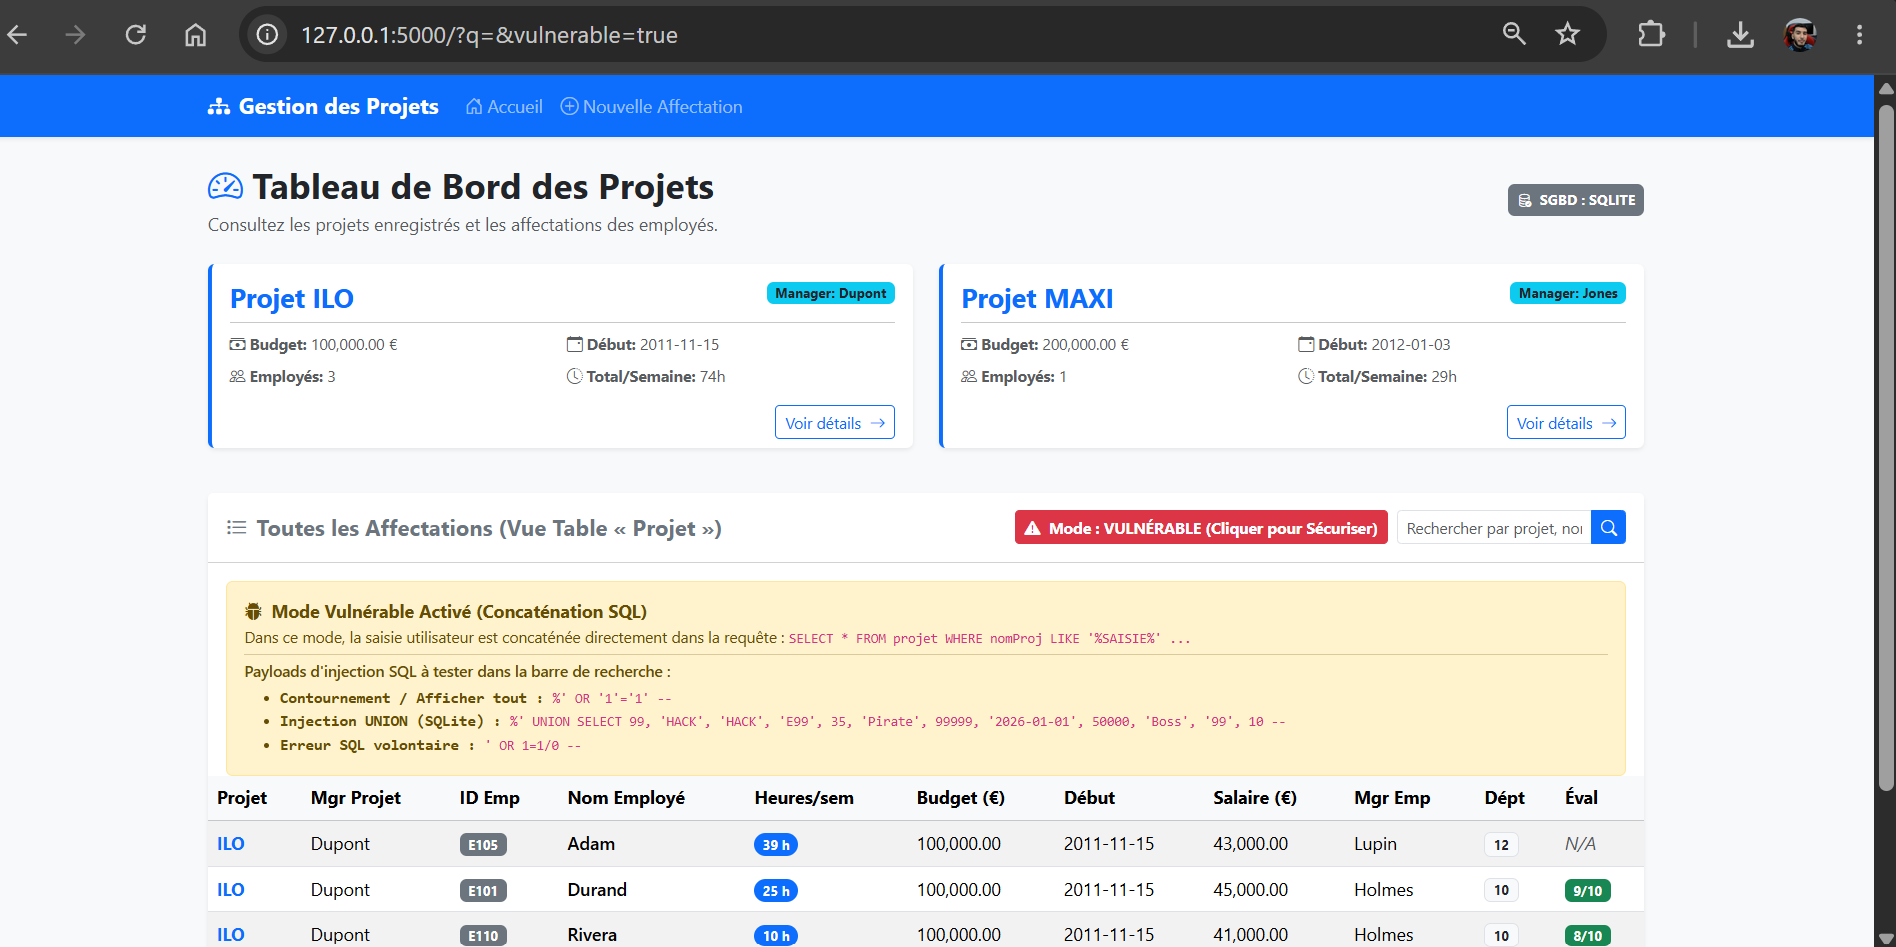
\includegraphics[width=0.9\textwidth]{capture_vulnerabilite.png}
    \caption{Capture d'écran de l'avertissement et des payloads d'injection SQL affichés dans l'application}
    \label{fig:notification_vulnerabilite}
\end{figure}

\begin{enumerate}
    \item \textbf{En Mode Vulnérable (Concaténation de chaînes) :}
    \begin{itemize}
        \item Le test avec \texttt{ILO'} provoque une erreur de syntaxe SQL (\textit{Unclosed quotation mark} / \textit{Syntax error}) car l'apostrophe casse la structure de la requête.
        \item Le test avec \texttt{\%' OR '1'='1' --} altère la logique de la clause \texttt{WHERE}, renvoyant \textbf{l'intégralité des enregistrements de la base de données}, y compris ceux des autres projets.
        \item Le test avec \texttt{UNION} permet d'injecter une ligne de données arbitraire (\texttt{Pirate}) affichée directement dans l'interface web.
    \end{itemize}

    \item \textbf{En Mode Sécurisé (Requêtes Paramétrées) :}
    \begin{itemize}
        \item Quel que soit le caractère ou le payload saisi (\texttt{ILO'}, \texttt{\%' OR '1'='1' --}), aucune erreur SQL n'est déclenchée.
        \item Le système recherche littéralement la sous-chaîne saisie. Comme aucun projet ne porte ce nom exact, l'application affiche simplement un tableau vide sans planter ni divulguer de données.
    \end{itemize}
\end{enumerate}

% --------------------------------------------------
\section{Analyse du code source}
% --------------------------------------------------
L'analyse du fichier source principal \texttt{app.py} permet de comprendre la différence fondamentale entre les deux modes de traitement des requêtes SQL.

\subsection{Code Vulnérable (Concaténation direct)}
Dans le mode vulnérable, la saisie utilisateur est directement intégrée dans la chaîne de la requête SQL par f-string Python :

\begin{lstlisting}[language=Python, caption=Code vulnérable à l'injection SQL]
# DANGEREUX : Concaténation directe de la saisie utilisateur
query_search = request.args.get("q", "")

sql_affectations = f"""
    SELECT * FROM projet
    WHERE nomProj LIKE '%{query_search}%'
       OR nomEmp LIKE '%{query_search}%'
       OR idEmp LIKE '%{query_search}%'
    ORDER BY nomProj, nomEmp;
"""
cursor.execute(sql_affectations) # Exécution directe
\end{lstlisting}

Ici, si \texttt{query_search} contient une apostrophe, celle-ci est interprétée comme un séparateur de chaîne SQL par le moteur de base de données.

\subsection{Code Sécurisé (Requêtes Paramétrées)}
Dans le mode sécurisé, l'application utilise des requêtes paramétrées avec des marqueurs d'emplacements (placeholders \texttt{?} ou \texttt{\%s}) :

\begin{lstlisting}[language=Python, caption=Code sécurisé prémuni contre l'injection SQL]
# SÉCURISÉ : Utilisation de requêtes paramétrées
query_search = request.args.get("q", "")
param_placeholder = "%s" if engine == "postgres" else "?"

sql_affectations = f"""
    SELECT * FROM projet
    WHERE nomProj LIKE {param_placeholder}
       OR nomEmp LIKE {param_placeholder}
       OR idEmp LIKE {param_placeholder}
    ORDER BY nomProj, nomEmp;
"""

search_pattern = f"%{query_search}%"
# Les données utilisateur sont passées dans le tuple en second argument
cursor.execute(sql_affectations, (search_pattern, search_pattern, search_pattern))
\end{lstlisting}

Le SGBD sépare la compilation de la structure de la requête et l'évaluation des valeurs des variables. La valeur fournie par l'utilisateur est donc traitée uniquement comme une donnée littérale.

% --------------------------------------------------
\section{Autres requêtes et opérations}
% --------------------------------------------------
La même méthodologie de sécurisation est appliquée sur l'ensemble des routes de l'application Flask, par exemple lors de l'affichage des détails d'un projet ou de l'insertion d'une nouvelle affectation :

\begin{lstlisting}[language=Python, caption=Requête paramétrée sur la vue détaillée d'un projet]
# Récupération sécurisée d'un projet par son nom
sql = f"SELECT * FROM projet WHERE nomProj = {param_placeholder} ORDER BY nomEmp;"
cursor.execute(sql, (nom_proj,))
affectations = cursor.fetchall()
\end{lstlisting}

De même pour l'insertion (\texttt{INSERT INTO}) dans la route \texttt{/affectation/nouvelle} :
\begin{lstlisting}[language=Python, caption=Insertion paramétrée sécurisée]
insert_sql = f"""
    INSERT INTO projet (nomProj, mgrProj, idEmp, heures, nomEmp, budget, dateDebut, salEmp, mgrEmp, deptEmp, evalEmp)
    VALUES ({', '.join([param_placeholder] * 11)});
"""
cursor.execute(insert_sql, (nomProj, mgrProj, idEmp, heures, nomEmp, budget, dateDebut, salEmp, mgrEmp, deptEmp, evalEmp))
\end{lstlisting}

% --------------------------------------------------
\section{Résultats des tests}
% --------------------------------------------------
Le tableau ci-dessous récapitule les comportements observés selon les entrées fournies et le mode d'exécution choisi :

\begin{table}[htbp]
\centering
\caption{Synthèse des résultats des tests d'injection SQL}
\vspace{0.2cm}
\begin{tabular}{|l|p{4cm}|p{4.5cm}|p{4.5cm}|}
\hline
\textbf{Test} & \textbf{Entrée / Payload} & \textbf{Résultat (Mode Vulnérable)} & \textbf{Résultat (Mode Sécurisé)} \\ \hline
Normal & \texttt{ILO} & Affiche les 3 affectations du projet ILO. & Affiche les 3 affectations du projet ILO. \\ \hline
Apostrophe & \texttt{ILO'} & Erreur de syntaxe SQL affichée / plantage. & Recherche du texte littéral \texttt{ILO'}, aucun résultat. \\ \hline
Contournement & \texttt{\%' OR '1'='1' --} & Affiche \textbf{toutes les lignes} de la table. & Recherche le texte littéral, aucun résultat. \\ \hline
UNION & \texttt{\%' UNION SELECT 99...} & Injecte une ligne arbitraire (\texttt{Pirate}) dans la table. & Recherche le texte littéral, aucun résultat. \\ \hline
\end{tabular}
\end{table}

% --------------------------------------------------
\section{Protection contre l'injection SQL}
% --------------------------------------------------
La principale protection mise en œuvre pour corriger cette vulnérabilité est l'utilisation systématique des \textbf{requêtes préparées ou paramétrées}.

Le mécanisme suit les étapes suivantes :
\begin{enumerate}
    \item Écrire la structure de la requête SQL avec des marqueurs d'emplacements (\texttt{?} en SQLite ou \texttt{\%s} en PostgreSQL/psycopg2) ;
    \item Transmettre la chaîne de requête et les paramètres sous forme de tuple ou de liste séparée à la méthode \texttt{cursor.execute()} ;
    \item Laisser le pilote de base de données échapper et gérer les types de données de manière totalement étanche.
\end{enumerate}

Il convient donc de proscrire impérativement la concaténation de chaînes de caractères (\texttt{+} ou \texttt{f"..."}) pour construire des requêtes SQL dynamiques contenant des entrées utilisateur.

% --------------------------------------------------
\section{Conclusion}
% --------------------------------------------------
Les tests réalisés sur l'application de gestion des projets ont permis d'analyser le comportement du serveur et du SGBD face à différentes entrées malveillantes.

Les expérimentations menées en mode vulnérable ont démontré qu'une simple concaténation de chaînes dans les requêtes SQL permet à un attaquant de contourner les filtres de recherche, d'extraire ou d'injecter des données non autorisées via la clause \texttt{UNION}.

En revanche, les tests menés en mode sécurisé confirment que l'utilisation des requêtes paramétrées avec \texttt{cursor.execute(sql, params)} neutralise totalement l'injection SQL. Les caractères spéciaux comme les apostrophes ou les mots-clés SQL sont traités uniquement comme de simples valeurs textuelles.

L'application respecte ainsi les recommandations de sécurité fondamentales en matière d'accès aux bases de données.

\end{document}
